\documentclass{article}
\usepackage[utf8]{inputenc}
\usepackage{amsmath}
\usepackage{graphicx}
\usepackage{float}
\usepackage{amssymb}
\usepackage{listings}
\usepackage{pgfplots}
\usepackage{siunitx}

\usepackage[table]{xcolor}
\usepackage{autotuwien}
\usepackage{tabularx}
\usepackage{ragged2e}
\usepackage{multirow}

\usepackage[printwatermark]{xwatermark}
\newwatermark[allpages,color=red!10,angle=45,scale=6,xpos=-1cm,ypos=1cm]{DRAFT}


% left justify footnotes
\usepackage[flushmargin,hang]{footmisc}
\renewcommand{\footnotelayout}{\raggedright}

\pgfplotsset{compat=1.15}
\title{ITIA Target Programming (Robot) Lab Report}
\author{Stefan Adelmann (01633044) and Hannes Brantner (01614466)}
\begin{document}
\maketitle{}
\clearpage{}
\section{SysML Review}

\section{I/O Mapping}

\subsubsection{Module}
\paragraph{Roboter}
Der Roboter verfügt über 6 Achsen und kann sich im 3D Raum frei bewegen. Positionen die angefahren werden sollen müssen durch Angabe von XYZ Koordinaten entweder erlernt oder im Programm zur Verfügung gestellt werden. Der Multifunktionsgripper besitzt Ausnehmungen um Kolben, Deckel und das Basisbauteil aufzunehmen. Die Farbe des Basisbauteils kann durch einen entsprechend eingestellten Reflektionssensor in binärer Weise (Bauteil nicht schwarz) erfasst werden.

\paragraph{Roboter Handling}
Das Handling Modul besteht aus einer Rutsche die Basis-Bauteile einer Abhohlposition zuführt. Bauteile werden in dieser Abhohlposition mittels eines Sensors erfasst und können vom Roboter aufgenommen werden. Als Ablagen stehen zwei Zylindermagazine sowie ein Ablageblock zur Verfügung.\newline
Eine Orientierungsausnehmung am Ablageblock ermöglicht das Ablegen und erneut aufnehmen des Basis-Bauteils. In der Montageausnehmung wird das Bauteil und die zusätzlichen Bestandteile zum Endprodukt vereint. \newline
Die Ortientierung des Basisbauteils bzw. des Deckels kann mittels einer Reflexlichtschranke erfasst werden. Die Rotation des Deckels erfolgt dabei um eine Rotationsachse die von einem passenden Metallstift vorgegeben ist.
\paragraph{Roboter Assembly}
%%\paragraph{6-Achs-Roboter RV-2FB}
Das Assembly Modul stellt Federn, Kolben und Deckel zur Verfügung. Das Federlager ist ein Zylinderlager aus dem mittels eines Schiebers Federn entnommen und angeboten werden. Ein Sensor ermittelt ob Federn zur Verfügung stehen, der Schieber kann pneumatisch aus und eingefahren werden. Im ausgefahrenen Zustand können Federn vom Roboter aufgenommen werden.\newline
Kolben werden dem Roboter auf einer Lochplatte mit zwei Reihen a 5 Kolben angeboten. Der Füllstand kann dabei nicht überprüft werden.\newline
Deckeln werden von einem pneumatischen Schieber aus einem Zylinderlager entnommen. Der Schieber befördert die Deckel in eine Ablageposition in der sie von einem Sensor erfasst werden. Der Schieber muss zur Aufnahme des Deckels eingefahren werden.\newline
Eine Rutsche dient als Ablage und Entnahmespunkt für fertiggestellte Bauteile.
\subsubsection{Sensoren/Aktoren}

\begin{center}
	\rowcolors{2}{white}{gray!25}
	\setlength\extrarowheight{4pt}
	\small
	\begin{tabularx}{\textwidth}{|p{4cm}|X|}
		\hline
		\rowcolor{tublau}
		\multicolumn{2}{|c|}{\bf \color{white} \large Sensoren}\\
		\hline\hline
		\rowcolor{gray!80}
		\bf Name & \bf Beschreibung\\
		\hline\hline
		RobPartOriented & Wert ist 1 wenn Bauteil ausgerichtet ist\\
		RobPartAvailable & Wert ist 1 wenn Bauteil vorhanden ist\\
		RobStart & Taster, Wert ist 1 wenn gedrückt\\
		RobStop & Taster, Wert ist 0 wenn gedrückt\\
		RobReset & Taster, Wert ist 1 wenn gedrückt\\
		RobSpringRetracted & Wert ist 1 wenn der Federschieber eingefahren ist\\
		RobSpringExtended & Wert ist 1 wenn der Federschieber ausgefahren ist\\
		RobSpringAvailable & Wert ist 1 wenn eine Feder vorhanden ist\\
		RobCapRetracted & Wert ist 1 wenn der Deckelschieber eingefahren ist\\
		RobCapExtended & Wert ist 1 wenn der Deckelschieber ausgefahren ist\\
		RobCapAvailable & Wert ist 1 wenn ein Deckel in der Abhohlposition liegt\\
		RobGripperNotBlack & Wert ist 1 wenn das Bauteil nicht schwarz ist\\
		\hline
	\end{tabularx}
	
	\medskip
	
	\begin{tabularx}{\textwidth}{|p{4cm}|X|}
		\hline
		\rowcolor{tublau}
		\multicolumn{2}{|c|}{\bf \color{white} \large Aktoren}\\
		\hline\hline
		\rowcolor{gray!80}
		\bf Name & \bf Beschreibung\\
		\hline\hline
		RobStartLed & Lampe leuchtet bei 1\\
		RobResetLed & Lampe leuchtet bei 1\\
		RobLed1 & Lampe leuchtet bei 1\\
		RobLed2 & Lampe leuchtet bei 1\\
		RobSpringPusher & Federschieber ausfahren\\
		RobCapPusher & Deckelschieber ausfahren\\
		\hline
	\end{tabularx}
\end{center}


\subsection{Roboter Steuerungs Komponenten}
\begin{center}
	%\scriptsize
	\setlength\extrarowheight{2pt}
	\begin{tabular}[t]{p{8cm}l}
		\rowcolors{2}{gray!25}{white}
		\begin{tabular}[t]{|p{1.2cm}p{4.5cm}|}
			\hline
			\rowcolor{gray} \multicolumn{2}{|c|}{\bf OPC UA Gateway}\\
			\hline\hline
			Device: & RaspberryPi 3\\
			ID: & BCM2835 (a02082)\\
			MAC: & b8:27:eb:09:db:ca\\
			IP: & 192.168.162.84/25\\
			\hline
		\end{tabular} &
		\rowcolors{2}{gray!25}{white}
		\begin{tabular}[t]{|p{1.2cm}p{5.5cm}|}
			\hline
			\rowcolor{gray} \multicolumn{2}{|c|}{\bf Controller}\\
			\hline\hline
			Device: & Robot Controller\\
			ID: & CR750-D\\
			MAC: & \\
			IP: & 192.168.162.82/25\\
			\hline
		\end{tabular} \\
	\end{tabular}
\end{center}
Sensoren werden über den Befehl \textbf{M\_In(<Index>)} in MELFA-BASIC V, bzw. in OPC UA über die Methode \textbf{readInput(<Index>)} mit der NodeId \textbf{ns=4;i=1075}, gelesen.
\begin{center}
	\rowcolors{2}{white}{gray!25}
	\setlength\extrarowheight{4pt}
	\small
	\begin{tabularx}{\textwidth}{|p{4cm}|X|}
		\hline
		\rowcolor{tublau}
		\multicolumn{2}{|c|}{\bf \color{white} \large Sensoren}\\
		\hline\hline
		\rowcolor{gray!80}
		\bf Index & \bf Beschreibung\\
		\hline\hline
		1 & Modul Roboterhandling - Werkstück ausgerichtet\\
		2 & Modul Roboterhandling - Werkstück in Abholposition\\
		3 & Bedienfeld - Start (Schließer)\\
		4 & Bedienfeld - Stopp (Öffner) \\
		5 & Bedienfeld - Reset (Schließer)\\
		7 & Bedienfeld - COM Brücke (I7)\\
		8 & Modul Robotermontage (Federmagazin) - Schieber eingefahren\\
		9 & Modul Robotermontage (Federmagazin) - Schieber ausgefahren\\
		10 & Modul Robotermontage (Federmagazin) - Feder vorhanden \\
		12 & Modul Robotermontage (Deckelmagazin) - Schieber eingefahren\\
		13 & Modul Robotermontage (Deckelmagazin) - Schieber ausgefahren\\
		15 & Modul Robotermontage (Deckelmagazin) - Deckel auf Ablage\\
		900 & Modul Roboter (Hand) - Teil nicht schwarz\\
		\hline
	\end{tabularx}
\end{center}
Aktoren werden über den Befehl \textbf{M\_Out(<Index>)=<value>} in MELFA-BASIC V, bzw. in OPC UA über den Befehl \textbf{writeOutput(<Index>,<value>)} mit der NodeId \textbf{ns=4;i=1075}, beschrieben.
\begin{center}
	\rowcolors{2}{white}{gray!25}
	\setlength\extrarowheight{4pt}
	\small
	\begin{tabularx}{\textwidth}{|p{4cm}|X|}
		\hline
		\rowcolor{tublau}
		\multicolumn{2}{|c|}{\bf \color{white} \large Aktoren}\\
		\hline\hline
		\rowcolor{gray!80}
		\bf Index & \bf Beschreibung\\
		\hline\hline
		0 & Bedienfeld - Start (LED)\\
		1 & Bedienfeld - Reset (LED)\\
		2 & Bedienfeld - Q1 (LED)\\
		3 & Bedienfeld - Q2 (LED)\\
		4 & Bedienfeld - COM Brücke (Q4)\\
		8 & Modul Robotermontage (Federmagazin) - Schieber ausfahren\\
		12 & Modul Robotermontage (Deckelmagazin) - Schieber ausfahren\\
		\hline
	\end{tabularx}
\end{center}

\begin{figure}[htp]
	\centering
	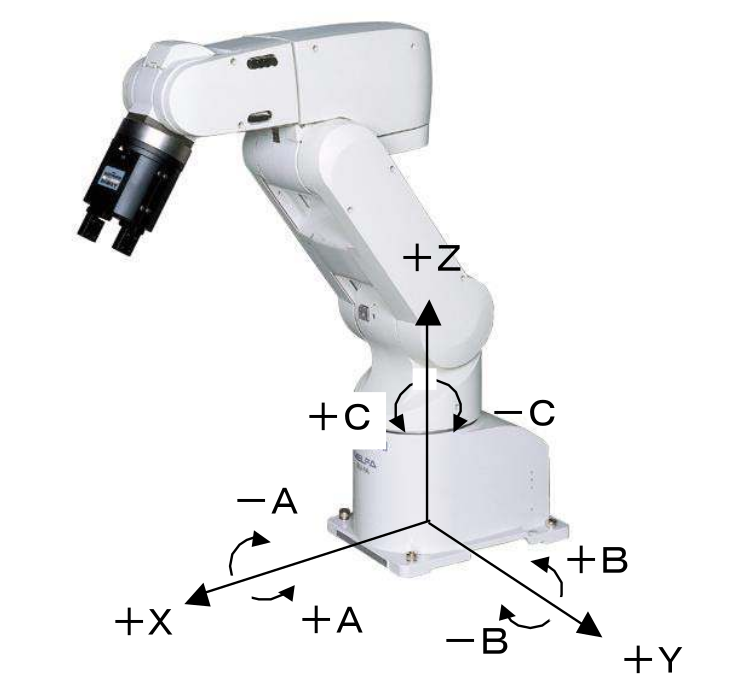
\includegraphics[width=0.6\textwidth]{images/robot_axis.png}
	\caption{Robot coordinate system in XYZ mode}
	\label{fig:robot_axis}
\end{figure}

\begin{center}
	\rowcolors{2}{white}{gray!25}
	\setlength\extrarowheight{4pt}
	\small
	
	\begin{tabularx}{\textwidth}{|p{3cm}|p{4cm}|X|}
		\hline
		\rowcolor{tublau}
		\multicolumn{3}{|c|}{\bf \color{white} \large Gripper}\\
		\hline\hline
		\rowcolor{gray!80}
		\bf Melfa-Command & \bf OPC UA & \bf Beschreibung\\
		\hline\hline
		Mov(X,Y,Z,A,B,C) & move(X,Y,Z,A,B,C) & Modul Roboter (Hand) - Position, Rotation anfahren\\
		HOpen 1 & gripperOpen() & Modul Roboter (Hand) - Gripper öffnen\\
		HClose 1 & gripperClose() & Modul Roboter (Hand) - Gripper schließen\\
		\hline
	\end{tabularx}
\end{center}



\section{Handover Protocol}


\end{document}
